%------------------------------------------------------------------------------------------------------------------------
\chapter{ローカルデータベースのブラウザ表示}
\label{sec:A}
%------------------------------------------------------------------------------------------------------------------------

%------------------------------------------------------------------------------------------------------------------------
\section{非読み出し試験結果のブラウザ表示}
\label{sec:A1}
%------------------------------------------------------------------------------------------------------------------------

\begin{figure}[h]
	\centering
	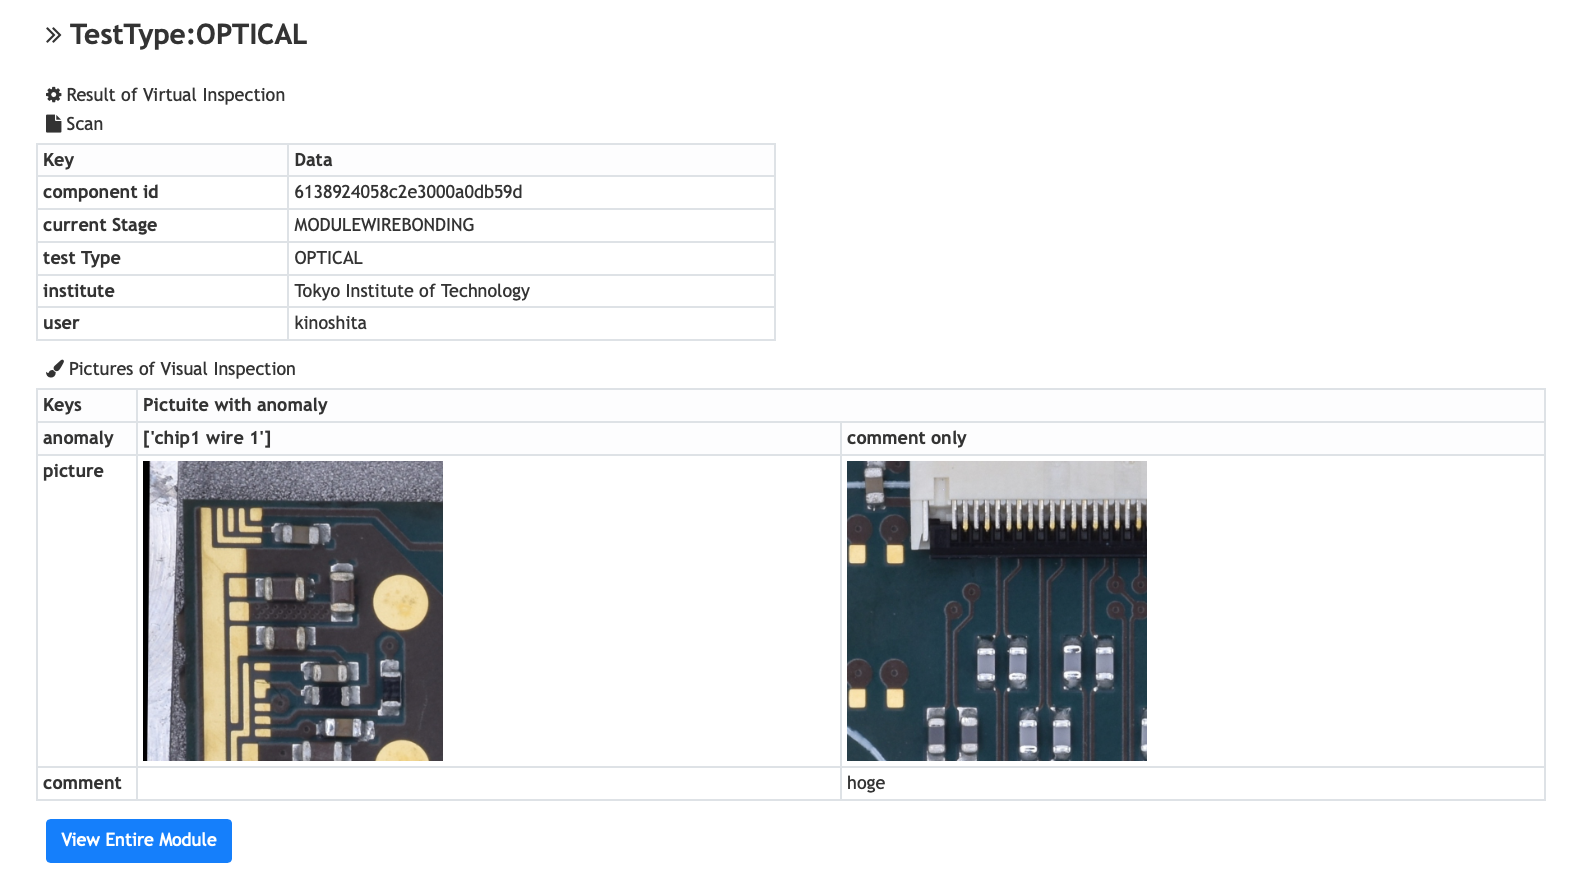
\includegraphics[height=8cm,keepaspectratio]{optical_pic.png}
	\caption[外観検査結果のブラウザ表示]{外観検査結果のブラウザ表示。}
	\label{fig:optical_pic}
\end{figure}

\begin{figure}[h]
	\centering
	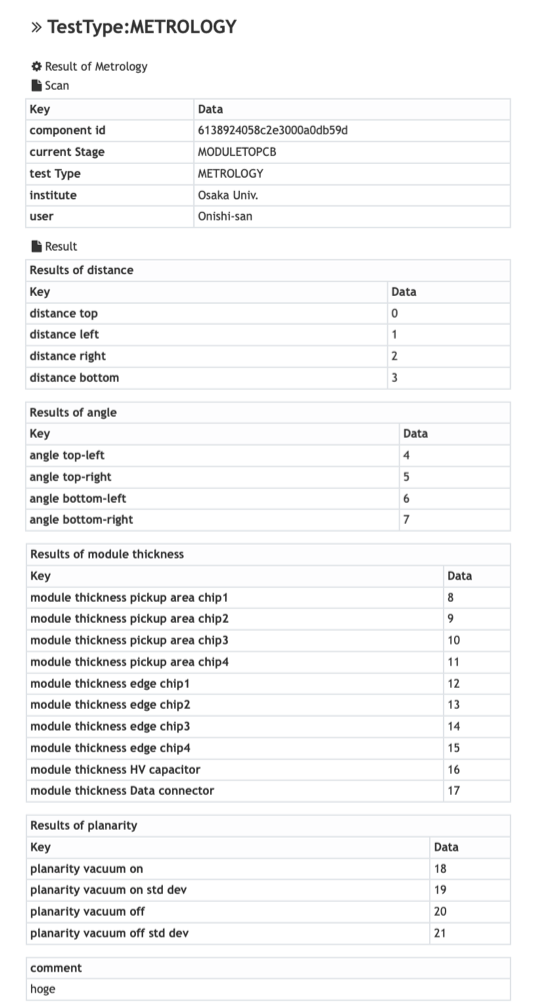
\includegraphics[height=16cm,keepaspectratio]{metrology_pic.png}
	\caption[平坦性測定結果のブラウザ表示]{平坦性測定結果のブラウザ表示。}
	\label{fig:metrology_pic}
\end{figure}


\begin{figure}[h]
	\centering
	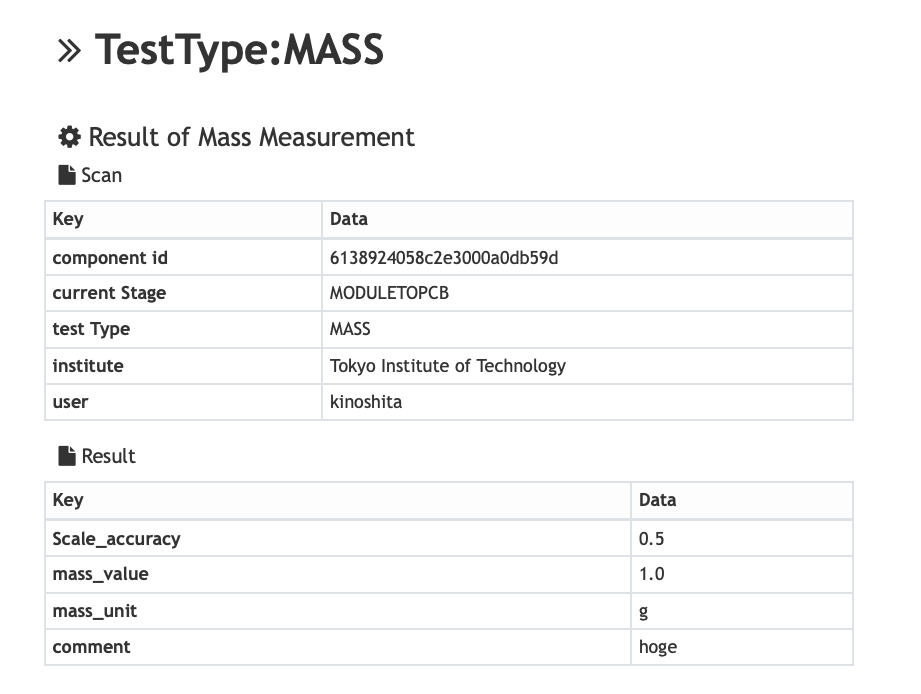
\includegraphics[height=8cm,keepaspectratio]{mass_pic.png}
	\caption[質量測定結果のブラウザ表示]{質量測定結果のブラウザ表示。}
	\label{fig:mass_pic}
\end{figure}

\begin{figure}[h]
	\centering
	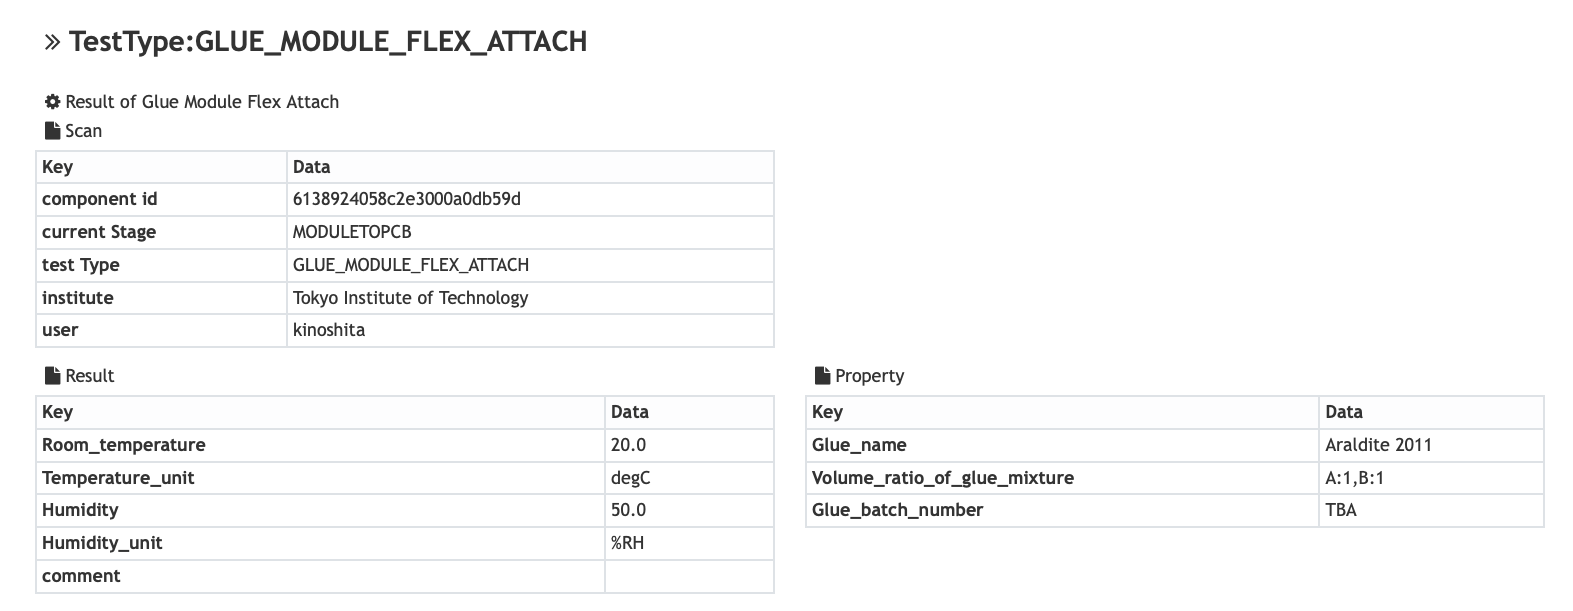
\includegraphics[height=6cm,keepaspectratio]{glue_pic.png}
	\caption[接着剤情報についてのブラウザ表示]{接着剤情報についてのブラウザ表示。}
	\label{fig:glue_pic}
\end{figure}

\begin{figure}[h]
	\centering
	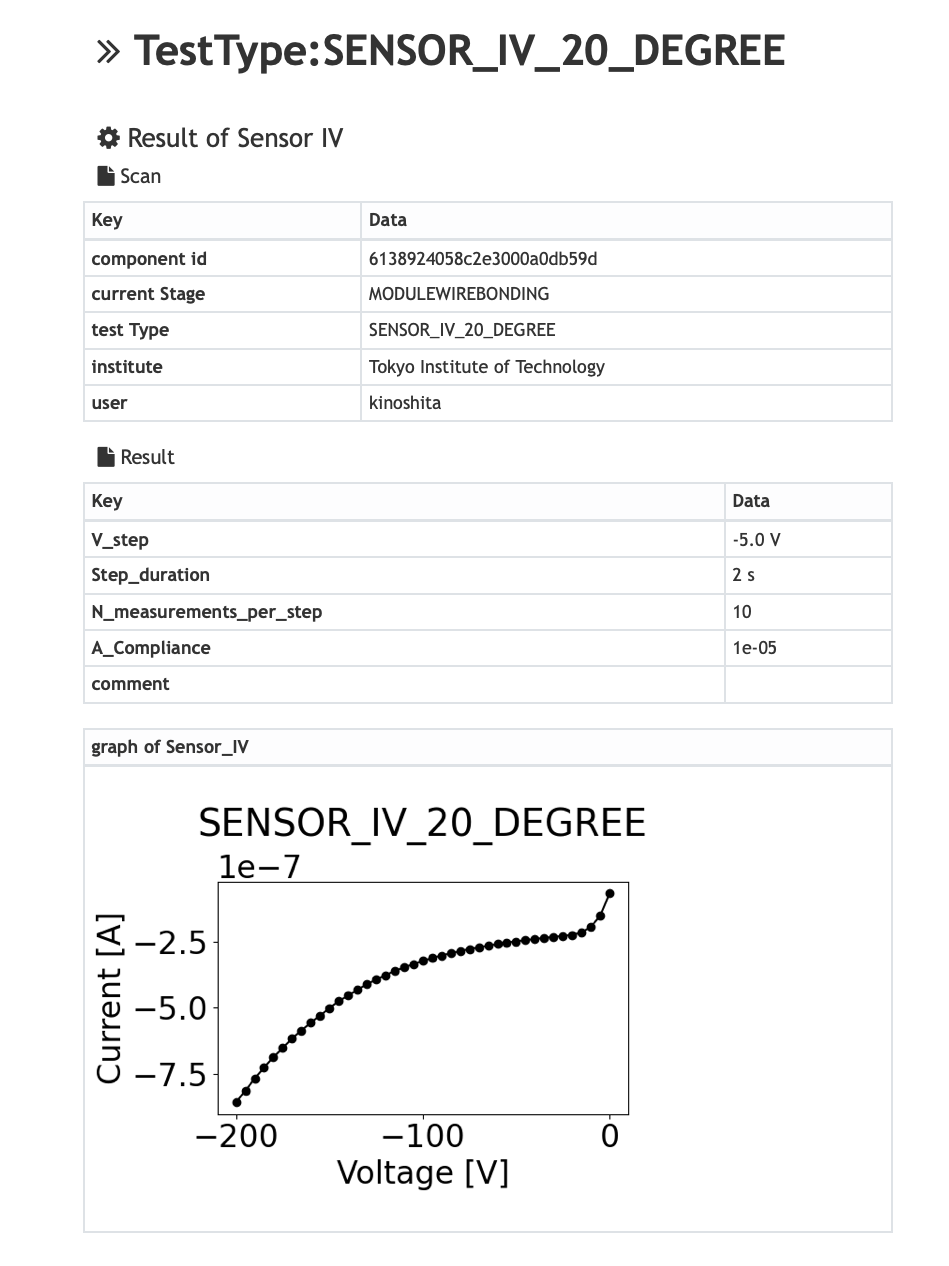
\includegraphics[height=9cm,keepaspectratio]{sensoriv_pic.png}
	\caption[センサー特性測定結果のブラウザ表示]{センサー特性測定結果のブラウザ表示。}
	\label{fig:sensoriv_pic}
\end{figure}

\begin{figure}[h]
	\centering
	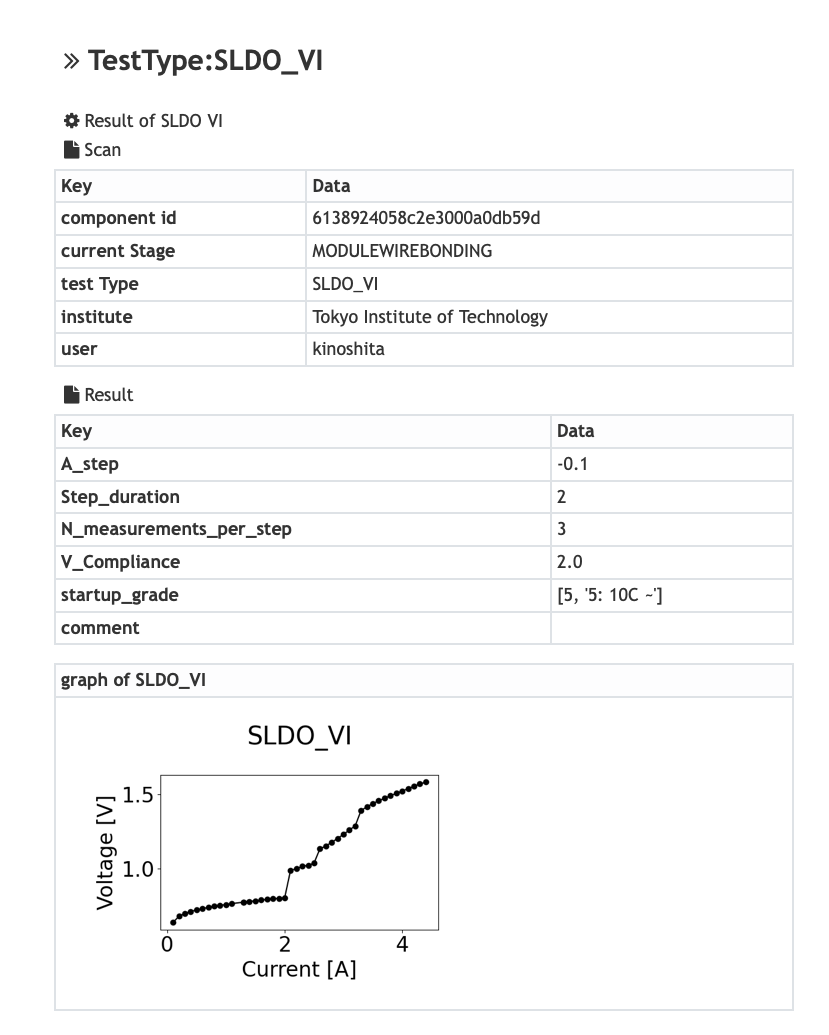
\includegraphics[height=9cm,keepaspectratio]{sldovi_pic.png}
	\caption[SLDO特性結果のブラウザ表示]{SLDO特性結果のブラウザ表示。}
	\label{fig:sldovi_pic}
\end{figure}

\begin{figure}[h]
	\centering
	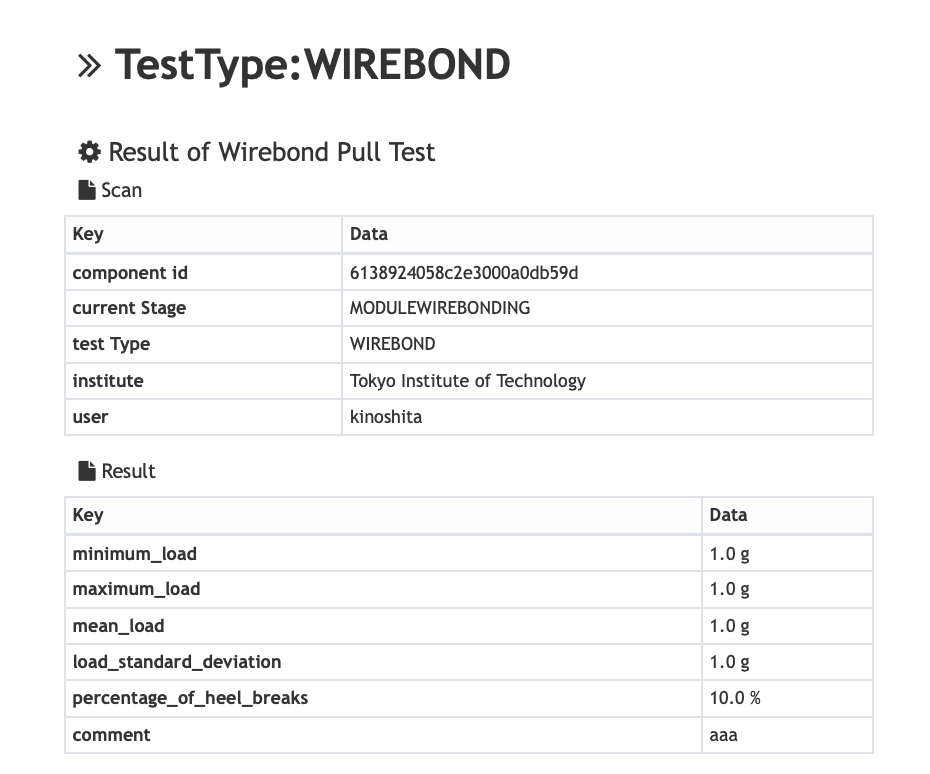
\includegraphics[height=7cm,keepaspectratio]{wirebondpull_pic.png}
	\caption[ワイヤー強度測定結果のブラウザ表示]{ワイヤー強度測定結果のブラウザ表示。}
	\label{fig:wirebondpull_pic}
\end{figure}

\begin{figure}[h]
	\centering
	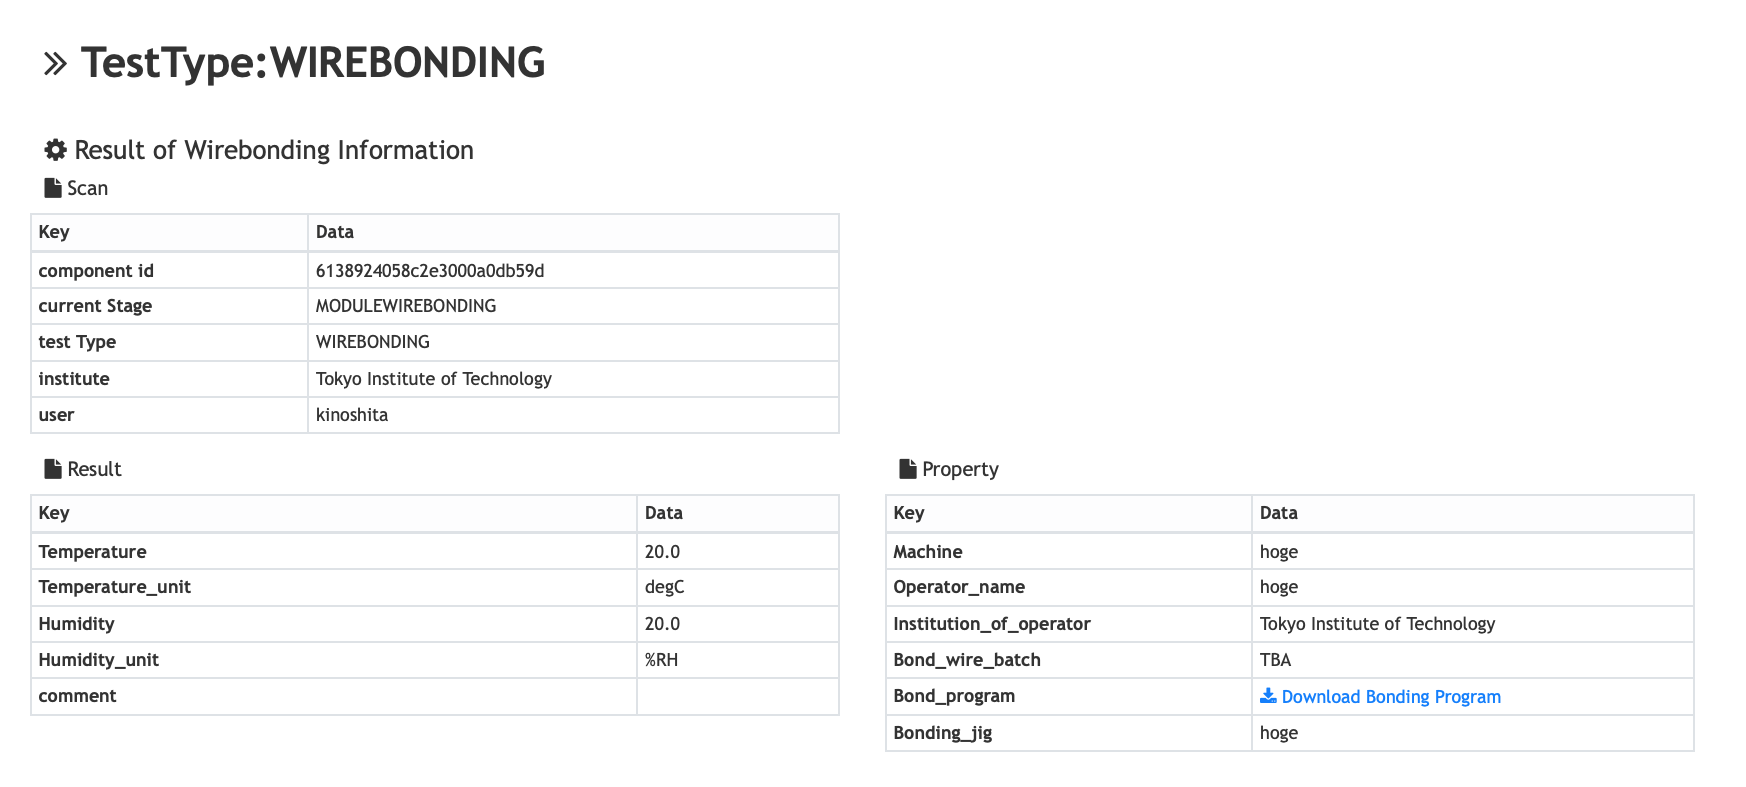
\includegraphics[height=6cm,keepaspectratio]{wireinfo_pic.png}
	\caption[ワイヤー配線情報のブラウザ表示]{ワイヤー配線情報のブラウザ表示。}
	\label{fig:wireinfo_pic}
\end{figure}



%------------------------------------------------------------------------------------------------------------------------
\section{ピクセルモジュール基本特性のブラウザ表示}
\label{sec:A2}
%------------------------------------------------------------------------------------------------------------------------


\begin{figure}[h]
	\centering
	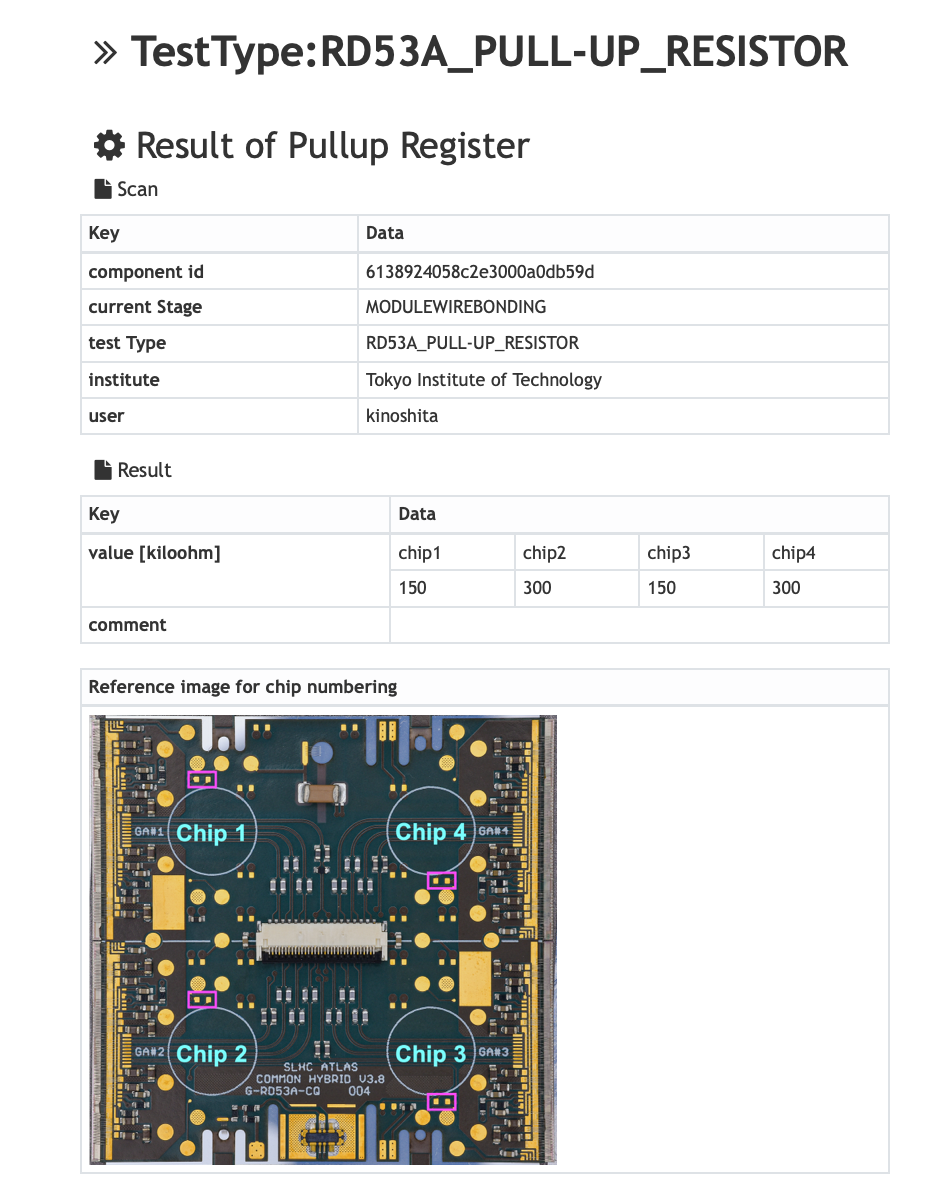
\includegraphics[height=9cm,keepaspectratio]{pullup_pic.png}
	\caption[プルアップ抵抗値のブラウザ表示]{プルアップ抵抗値のブラウザ表示。}
	\label{fig:pullup_pic}
\end{figure}

\begin{figure}[h]
	\centering
	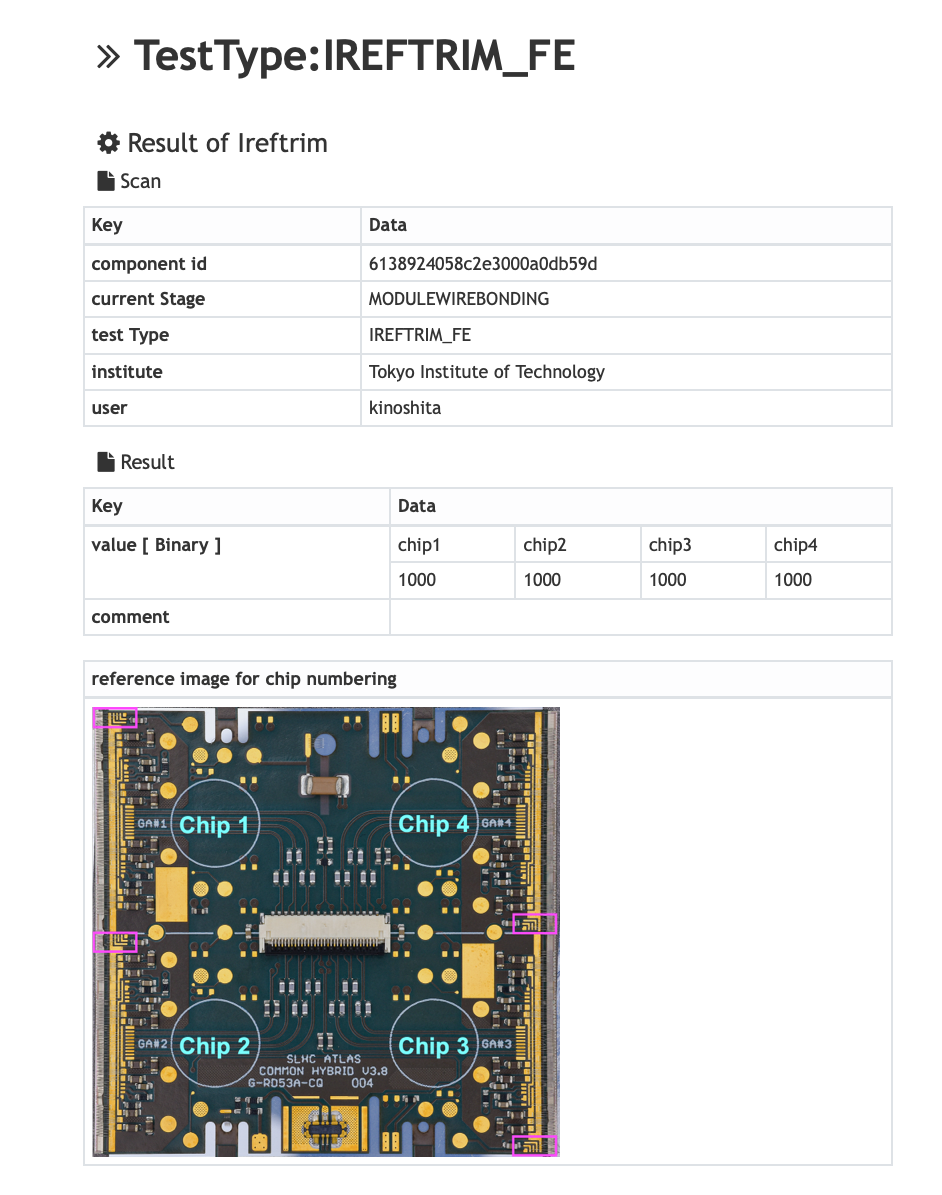
\includegraphics[height=9cm,keepaspectratio]{iref_pic.png}
	\caption[IrefTrim値のブラウザ表示]{IrefTrim値のブラウザ表示。}
	\label{fig:iref_pic}
\end{figure}

\begin{figure}[h]
	\centering
	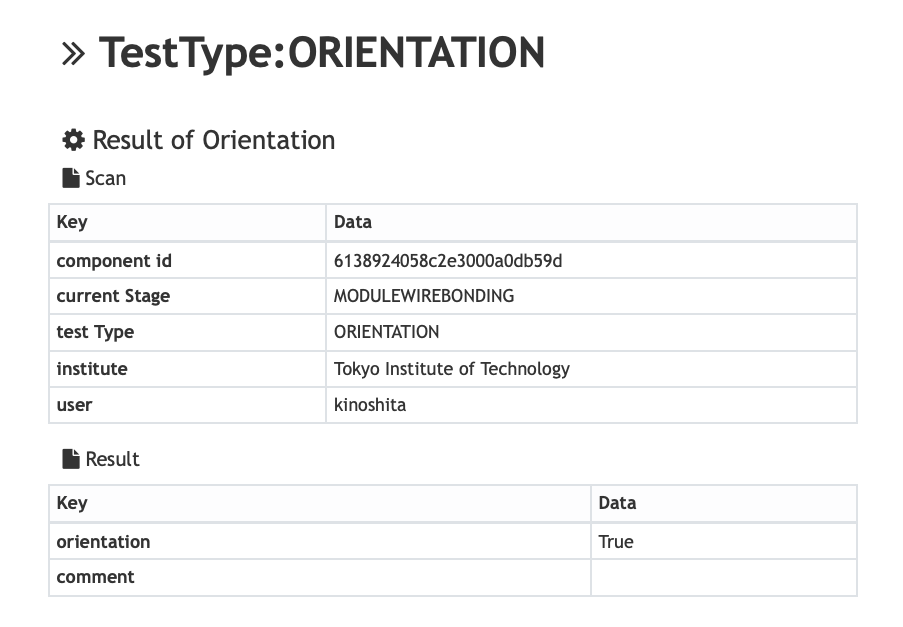
\includegraphics[height=7cm,keepaspectratio]{orientation_pic.png}
	\caption[ベアモジュールとフレキシブル基板の向きについてのブラウザ表示]{ベアモジュールとフレキシブル基板の向きについてのブラウザ表示。}
	\label{fig:orientation_pic}
\end{figure}
